% !TeX root = f61_longreport_schmitt_kleinbek.tex
\section{Theoretical Basics}



\subsection{Basics and the relaxation time}
In an applied external magnetic field, existing magnetic moments of the atomic nuclei in a material align themselves along the external magnetic field, parallel or anti-parallel.
The corresponding energy splitting is given by the scalar product of magnetic moment and external magnetic field in the form
\begin{align}
\Delta E=-\vec{\mu}\cdot\vec{B}_0.
\end{align}
The parallel alignment is energetically lower.\\
The proton population numbers correctly described by the Fermi-Dirac statistics can be approximated classically by the Boltzmann distribution.
The ratio of the two occupation numbers with parallel and antiparallel alignment is then given by
\begin{align}
\frac{N_+}{N_-}=\e{\frac{2\Delta E}{k_\text{B}T}}.
\end{align}
An estimate in which the magnetic moment is approximately one Bohr's magneton and the magnetic field is approximately \SI{1}{\tesla} results in a difference between the two occupation numbers of approximately one per thousand at room temperature.\\
The total magnetization results from the sum of these thousandth part over the whole substance.
In general, the following applies from the electrodynamics for the resulting torque from a magnetic field and a magnetization
\begin{align}
\vec{\tau}=\vec{M}\times\vec{B}_0.
\end{align}
For (anti-)parallel alignment, the torque is zero.
As soon as $B_0$ and $M$ span a plane, the resulting torque rotates the magnetization around the axis of the magnetic field with the Larmor frequency
\begin{align}
\omega_\text{L}=\gamma\,B_0.
\label{eq:lamor}
\end{align}
Now we create a second magnetic field $B_1$ orthogonal to a relatively strong external magnetic field $B_0$.
Before the magnetization can align itself along the new total magnetic field $B_\text{tot}$, the Larmor precession around this begins.
If the magnetic field $B_1$ oscillates with the Larmor frequency of the atomic nuclei, the magnetization can be deflected, as schematically shown in Figure \ref{fig:magnet}.
\begin{figure}[ht]
\centering
% !TeX root = ..//f61_longreport_schmitt_kleinbek.tex
\begin{tikzpicture}[scale=.75]
\draw[arrows=-{Stealth[scale=.75]}, ultra thick, color=grey] (0,0)--+(0,4) node [above]{$B_0$};
\draw[arrows=-{Stealth[scale=.75]}, line width=1mm, color=myred] (0,0)--+(0,2) node [left]{$M$};
\fill (0,0) circle (1.9pt)[color=myred];

\draw [thick, rotate=-23](3.7,3.43) ellipse (.8cm and .4cm);
\draw[arrows=-{Stealth[scale=.75]}, ultra thick, color=grey] (4,0)--+(0,4) node [above]{$B_0$};
\draw[arrows=-{Stealth[scale=.75]}, ultra thick, color=grey, dashed] (4,0)--+(1.5,0) node [below]{$B_1$};
\draw[arrows=-{Stealth[scale=.75]}, line width=.75mm] (4,0)--+(1.5,4) node [right]{$B_\text{tot}$};
\draw[arrows=-{Stealth[scale=.75]}, line width=1mm, color=myred] (4,0)--+(0,2) node [left]{$M$};
\fill (4,0) circle (1.9pt)[color=myred];

\draw [thick, rotate=18](11.3,-2.8) ellipse (1.9cm and .4cm);
\draw[arrows=-{Stealth[scale=.75]}, ultra thick, color=grey] (12,0)--+(0,4) node [above]{$B_0$};
\draw[arrows=-{Stealth[scale=.75]}, ultra thick, color=grey, dashed] (12,0)--+(-1.5,0) node [below]{$B_1$};
\draw[arrows=-{Stealth[scale=.75]}, line width=.75mm] (12,0)--+(-1.5,4) node [left]{$B_\text{tot}$};
\draw[arrows=-{Stealth[scale=.75]}, line width=1mm, color=myred] (12,0)--+(45:2) node [right]{$M$};
\fill (12,0) circle (1.9pt)[color=myred];
\end{tikzpicture}
\caption{High-frequency external magnetic field generates elongation of magnetization.}
\label{fig:magnet}
\end{figure}
With the duration of the applied high-frequency magnetic field $B_1$ we can determine the angle by which the magnetization is deflected compared to the external magnetic field $B_0$.
In particular, so-called $\ang{90}$ and $\ang{180}$ pulses can be generated, which generate an orthogonal or antiparallel magnetisation to $B_0$ from a parallel magnetisation.\\

For these excited states of magnetization, the Bloch equations result in an asymptotic drop on characteristic time scales for antiparallel and orthogonal magnetization respectively $T_1$ and $T_2$:
\begin{align}
M_\parallel(t)&=M_0\cdot\left(1-2\e{-\frac{t}{T_1}}\right)\\
M_\bot(t)&=M_0\cdot\e{-\frac{t}{T_2}}
\end{align}
The decay of the anti-parallel magnetization is caused by the interaction of the spins with the external magnetic field $B_0$ (spin-grating changer effect), whereas interactions between the individual spins (spin-spin interaction) lead to the decay of the parallel magnetization.
Since the spin-spin interaction is stronger than the spin-grating interaction, $T_2\leq T_1$ is expected.\\
Measurements of orthogonal magnetization are made in the $B_1$ generating coil by induction.
After switching off the $B_1$ field, the precession of the magnetization around the external magnetic field $B_0$ induces an alternating current in the $B_1$ coil.
This can be measured on a connected oscilloscope.
In our setup, the output signal of the induction coil leads back again into the signal generator, which generates the high-frequency alternating field $B_1$, and only then into the readout devices.
Thus we see the final signal as a superposition of the signal frequency and the alarm frequency, which shows the sum and difference of the two frequencies.
We also call the difference the operating frequency, which is a few hundred hertz; this difference is in the per thousand range relative to the larmor frequency of hydrogen nuclei (about \SI{20}{\mega\hertz}).\\

The relaxation time $T_1$ can be measured by first passing a $\ang{180}$ pulse
an antiparallel orientation of the magnetization is caused and then after different time intervals a $\ang{90}$ pulse generates a signal in the induction coil whose amplitude is proportional to the magnitude of the antiparallel magnetization of before the $\ang{90}$ pulse.
By recording these amplitudes after different times, the exponential decrease of the antiparallel magnetization can be investigated and $T_1$ determined.\\

The relaxation time $T_2$ is measured by another combination of $\ang{90}$ and $\ang{180}$ pulses.
First a $\ang{90}$ pulse produces a magnetization perpendicular to the $B_0$ field, which because of this field begins to precisionize this axis with the Larmor frequency.
However, the external magnetic field is designed so that the magnetic field strength varies in the direction of the magnetic field vector.ends on it, the frequency at different coordinates is also different, which after a certain time results in a phase diff
Because the Larmor frequency by equation \ref{eq:lamor} deperence at the different coordinates.
This incoherence reduces the amplitude of the induced field in the coil.
After a certain period of time $\tau$ a $\ang{180}$ pulse is sent, which causes a mirroring around $\ang{180}$ on an axis perpendicular to the axis of the $B_0$ field around which the magnetization rotates.
The consequence of this mirroring is that the nuclei that were previously in phase after the other nuclei are now at the same phase angle in front of them. 
The previous phase difference was due to the precession during a time $\tau$ had arisen.
By mirroring through the $\ang{180}$ pulse, after a further precession period of $\tau$, the nuclei are all in phase again and thus show a maximum induction current.
This allows the magnitude decrease to be measured over a period of 2$\tau$ .\\
Now you can always use different values for $\tau$ and measure the decrease of the amplitude after twice the time to reconstruct the exponential decrease and so $T_2$.
\begin{figure}[ht]
\centering
% !TeX root = ..//fp_nmr_schmitt_kleinbek_18.tex
\begin{tikzpicture}[scale=.7]
%point
\foreach \i in {4.5,9}
\fill (\i,0) circle (2pt);

%circle
\foreach \i in {0,4.5,9,13.5}
\draw [thick] (\i,0) circle (1cm);

%time
\node at (0,2.5){$t=0$};
\node at (4.5,2.5){$t=\tau$};
\node at (9,2.5){$t=\tau$};
\node at (13.5,2.5){$t=2\tau$};
\node at (1.2,1.25)[color=grey]{$\ang{90}$-Puls};

%coordinates
\foreach \i in {0,4.5,9,13.5}
\draw[arrows=-{Stealth[scale=1]},thick](\i,0)--+(0,1.5) node[left]{$x$};
\foreach \i in {0,4.5,9,13.5}
\draw[arrows=-{Stealth[scale=1]},thick](\i,0)--+(1.5,0) node[below]{$y$};

%timearrows
\draw[arrows=-{Stealth[scale=.75]}, color=grey, line width=.75mm](2,0)--+(1,0) node[midway, above]{$\tau$};
\draw[arrows=-{Stealth[scale=.75]}, color=grey, line width=.75mm](6.5,0)--+(1,0) node[midway, above]{$\ang{180}$};
\draw[arrows=-{Stealth[scale=.75]}, color=grey, line width=.75mm](11,0)--+(1,0) node[midway, above]{$\tau$};

%arrows
\draw[arrows=-{Stealth[scale=.5]}, color=myred, line width=1.25mm](0,0)--+(1.2,0) node[midway, below, xshift=-3pt]{\footnotesize $M_\bot$};
\draw[arrows=-{Stealth[scale=.5]}, color=myred, line width=1.25mm](13.5,0)--+(-1.2,0) node[midway, below, xshift=3pt]{\footnotesize $M_\bot$};
\draw[arrows=-{Stealth[scale=1]},thick](4.5,0)--+(-35:1.5) node[below]{$\omega_2$};
\draw[arrows=-{Stealth[scale=1]},thick](4.5,0)--+(-60:1.5) node[below]{$\omega_1$};
\draw[arrows=-{Stealth[scale=1]},thick](9,0)--+(215:1.5) node[below]{$\omega_2$};
\draw[arrows=-{Stealth[scale=1]},thick](9,0)--+(240:1.5) node[below]{$\omega_1$};

\draw[arrows=-{Stealth[scale=1]},thick, shift = {(0.8,-0.8)}](5.42,-.4) arc (-25:-80:1);
\draw[arrows=-{Stealth[scale=1]},thick, shift = {(-0.8,-0.8)}](8.8,-.97) arc (-100:-155:1);

%redcircle
\foreach \i in {0,13.5}
\fill (\i,0) circle (1.775pt)[color=myred];
\end{tikzpicture}
\caption{Diagram for measuring the relaxation time $T_2$.}
\label{fig:relaxation}
\end{figure}
This measuring method is called spin-echo method.\\

Alternatively, another $\ang{180}$ pulse can be sent to all odd multiples of time $\tau$ so that a maximum induction current is measured at all even multiples of $\tau$ and the relaxation time can be determined from this.
This sequence of one $\ang{90}$ and several $\ang{180}$ pulses is called the Carr-Purcell sequence.
The basic procedure of the process described here is shown in figure \ref{fig:relaxation} is illustrated.



\subsection{Chemical Shift}
When considering the excitation of nuclear spins, only atoms that actually have a nuclear spin can be excited (i. e. $S\neq 0$).
Of course, a single proton as fermion in the nucleus of a hydrogen atom has a spin of $S = \nicefrac{1}{2}$.
On the other hand, for a carbon atom, for example, $S = 0$, so there is no magnetic moment at all that could contribute to magnetization.\\
Additionally, note that the $\ang{90}$ and $\ang{180}$ pulses are always adjusted to a noise frequency.
In order to achieve an effective excitation of nuclear spins of different atoms, the gyromagnetic ratio must also be the same.
If we expose a sample of organic material to only one frequency that excites hydrogen nuclei, only the hydrogen atoms of an organic material will contribute to the measured larmor frequency.
In different molecules the hydrogen molecules are present in different bonds with different electronegativity differences, which means that the probability of residence of the electrons around the proton is not always the same.
Due to this difference, the externally applied magnetic field $B_0$ is also shielded to different degrees by the electron, which results in a slightly different larmor frequency.
The shielded part of the magnetic field is described by
\begin{align}
\delta\vec{B}=-\sigma\vec{B}_0,
\end{align}
where $\sigma$ is the proportionality factor.
For a certain material, the changed Larmor frequency results accordingly from the superposition of both magnetic fields to
\begin{align}
\omega_i=\omega_\text{L}(1-\sigma_i).
\end{align}
In order to identify a sample on the basis of this shift of the Larmor frequency, the shielding factors relative to a reference sample (here Tetra-Methyl-Silane, short TMS) are measured by measuring the distance of the corresponding resonance peaks.
This distance then corresponds to
\begin{align}
\delta_i\cdot\omega_\text{L}=\omega_\text{TMS}-\omega_i.
\end{align}
The differences of the shielding factors $\delta_i =\sigma_i-\sigma_\text{TMS}$ can then be looked up in a table as shown in figure \ref{fig:shift}.\\
The positions of the molecules in this list can be explained using the example of a COOH group.
\begin{figure}[ht]
\centering
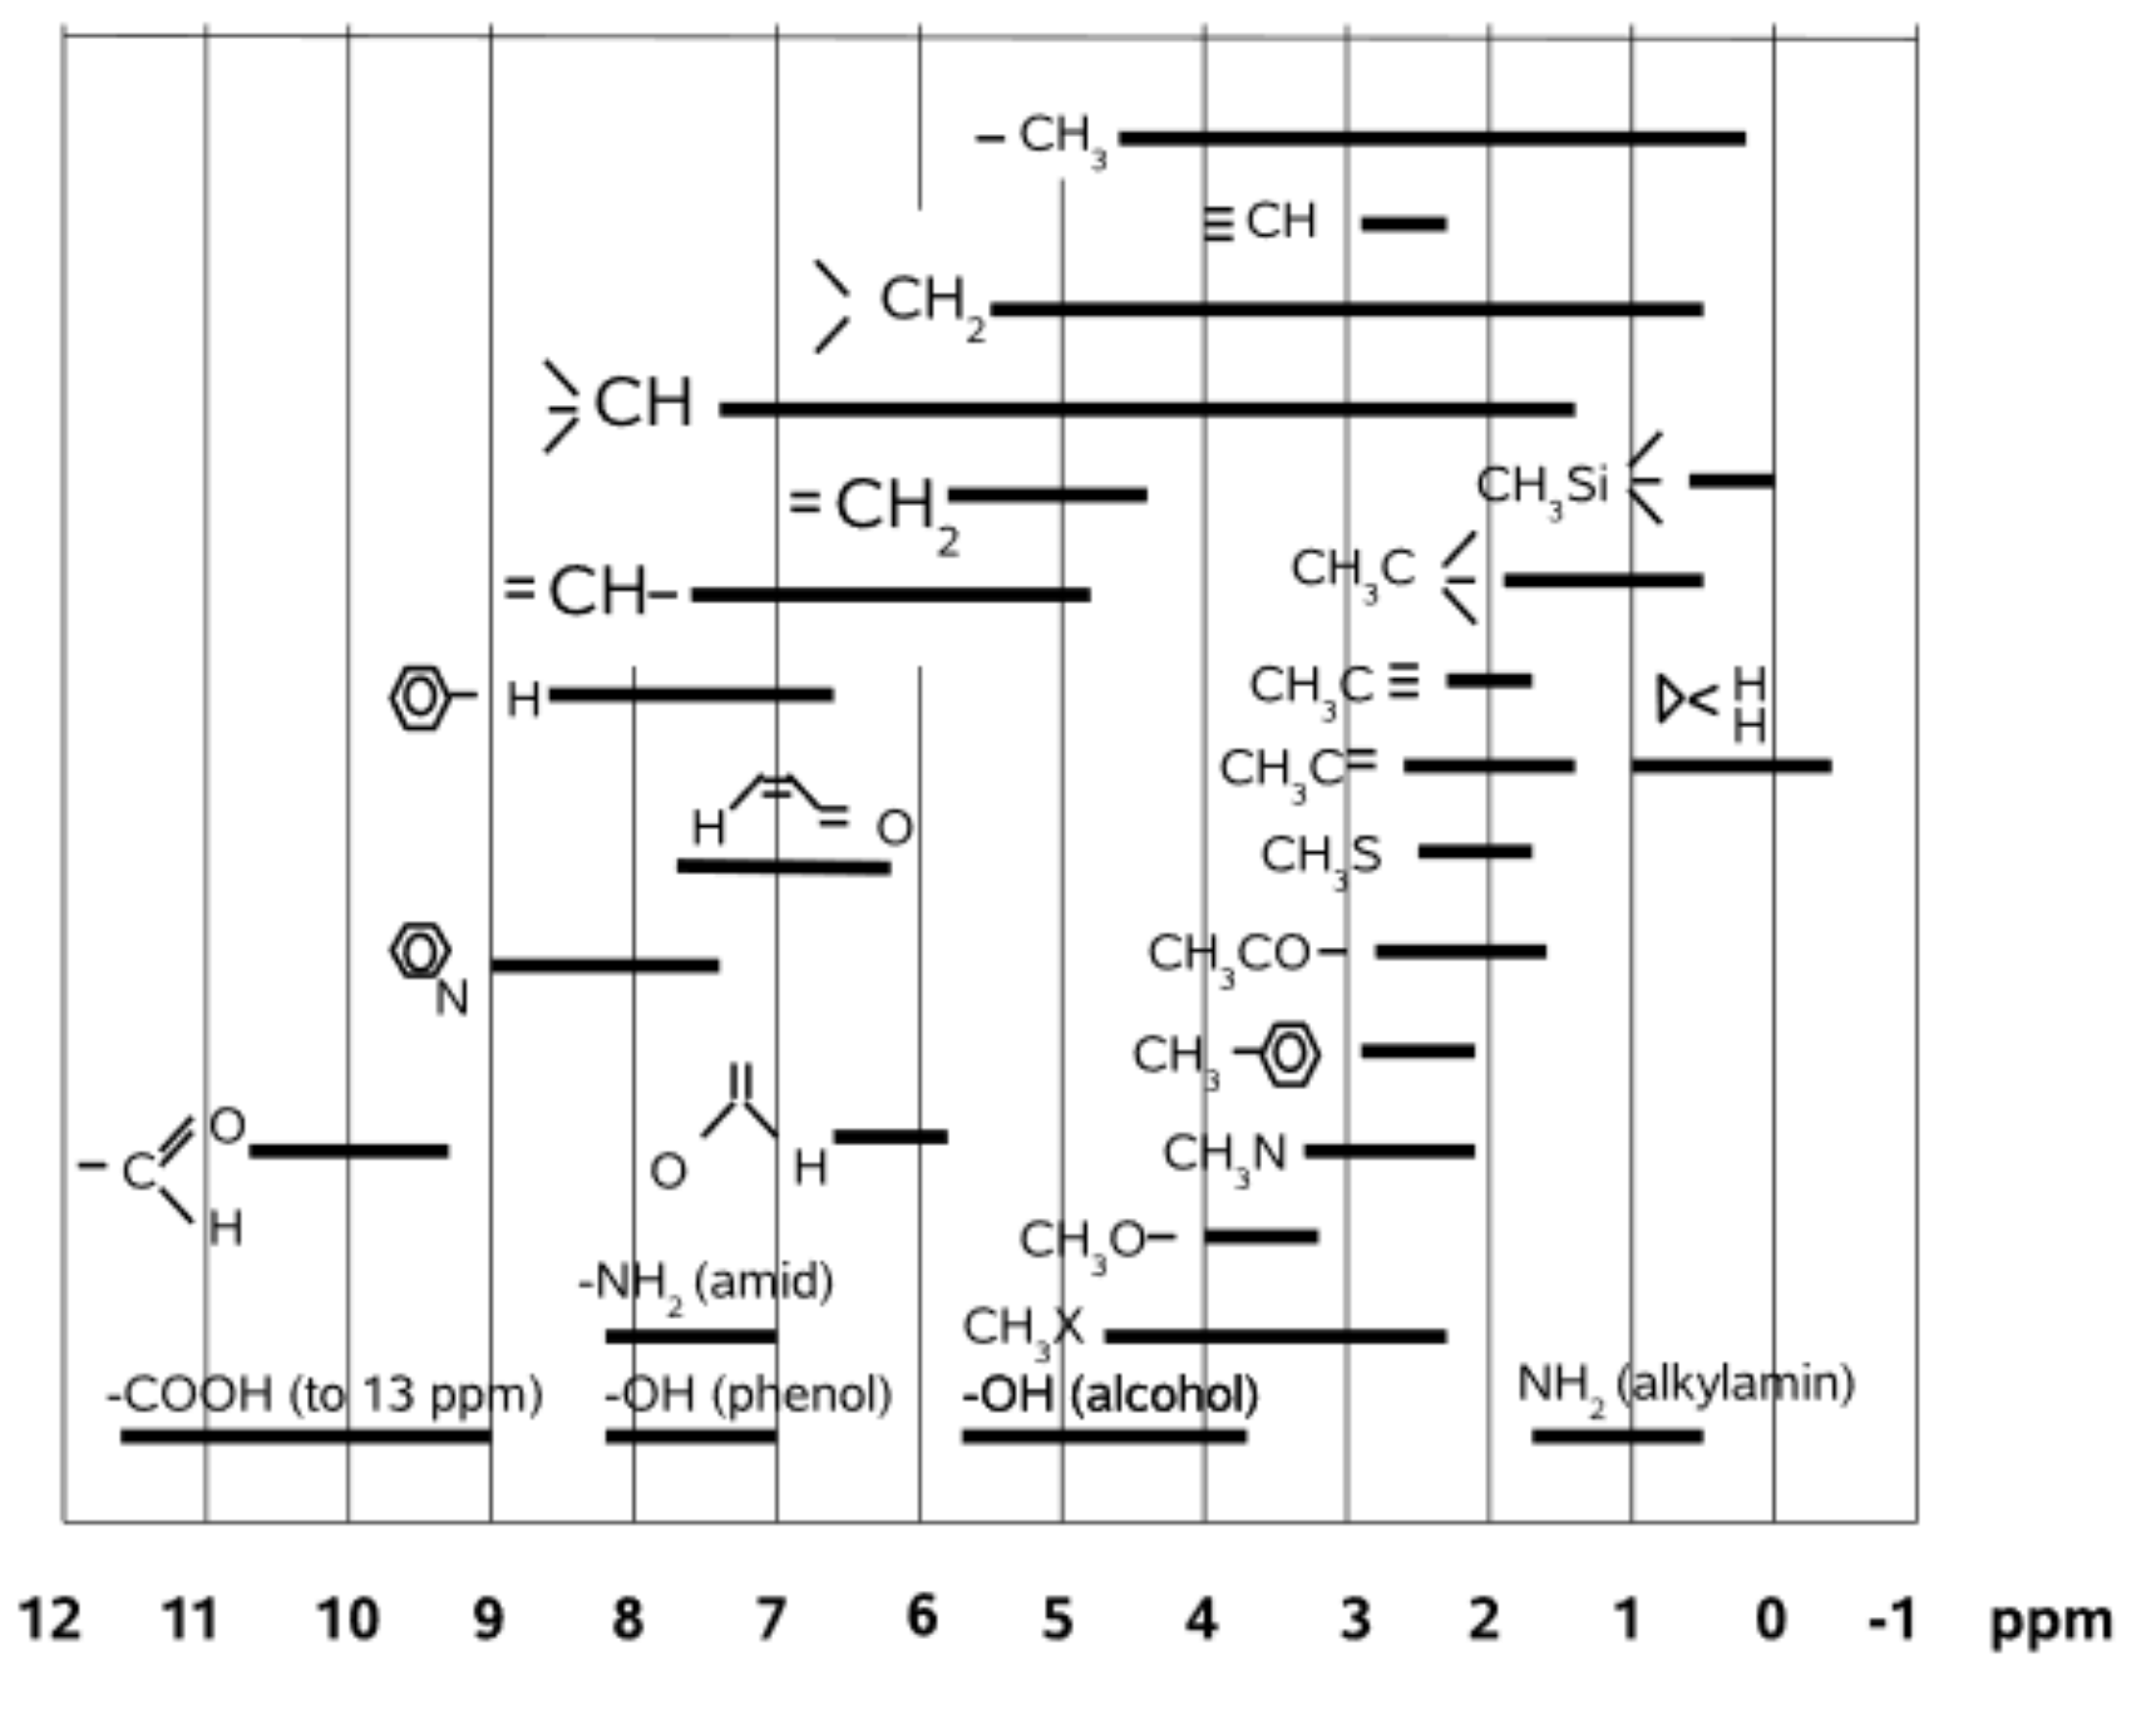
\includegraphics[scale=.175]{images//shift.png}
\caption{Chemical shifts of different molecules relative to TMS \cite{script_nmr}.}
\label{fig:shift}
\end{figure}
Here, the hydrogen atom is directly bonded to an oxygen atom with a relatively high electronegativity, while a second oxygen atom is bonded directly to an oxygen atom with a relatively high electronegativity.
oxygen atom is still in the immediate vicinity.
The hydrogen atom itself is thus virtually \enquote{naked} and is hardly shielded from its electron, which leads to a stronger effective magnetic field compared to C-H bonds and thus to an increased larmor frequency. 



\subsection{Imaging Techniques}
By excitation of nuclear spins and subsequent measurement of the magnetization, the distribution of the excited spins can be reconstructed under certain conditions and thus one-, two- or three-dimensional images of the nuclear spin distribution can be generated.
To divide the material into readable pixels in the different dimensions, in addition to an external $B_0$ field along the direction, which we now define as $z$ direction, we use magnetic fields, which also point in $z$ direction but change spatially with the $x, y$ or $z$ coordinate.
In $x$ direction, for example:
\begin{align*}
\vec{B}_x=(0,0,G_xx)
\end{align*}

\subsubsection{Frequency Coding}
After equation \ref{eq:lamor} the Larmor frequency in a magnetic field, which is superimposed by $B_0$ and a field varying in $z$ direction, results to
\begin{align}
\omega_\text{L}(z)=\gamma(B_0+G_zz)=\omega_\text{L}^0+\omega_z.
\end{align}
As soon as a $\ang{90}$ pulse causes a magnetization in the $x-y$ plane, this precedes the $z$ position with different alarm frequency around the axis of the magnetic field.
The signal generated in an adjacent induction coil whose axis must be perpendicular to the $z$ direction is then proportional to the sum of all magnetizations multiplied by the phase resulting from the high frequency of the $\ang{90}$ pulse
\begin{align}
S(t)&\sim\int\limits_V M_\bot(z,t)\,\e{-\im\omega_\text{HF}t}\dd{V}\\
\intertext{what is equal to}
S(t)&\sim\int\limits_V M_\bot^\text{rot}(z,t)\,\e{-\im\left(\omega_\text{L}^0+\omega_z-\omega_\text{HF}\right)t}\dd{V}.
\end{align}
If we assume that $\Omega=\omega_\text{L}^0-\omega_\text{HF}$, the exponential function before the integral only contributes a phase and we get
\begin{align}
S(t)&\sim\e{\im\Omega t}\int\limits_Z\left(\int\limits_X\int\limits_Y M_\bot^\text{rot}(z,t)\dd{y}\dd{x}\right)\e{\im\omega_z t}\dd{z}.
\end{align}
After integration over the area of the induction coil, the measured signal is thus proportional to the Fourier transform of the magnetization.
By measuring the signal at different times $t_i$ the distribution of the magnetization depending on the position $z$ can be calculated by discrete Fourier transformation.
As usual for functions that are linked via Fourier transform, the product of characteristic widths of the functions is constant.\\
Therefore, the following applies
\begin{align}
\Delta z\sim\frac{1}{\Delta t}.
\end{align}
The nuclear spins along the $z$ coordinate have because of the inhomogeneous magnetic field different Larmor frequencies and the information of the position is \enquote{encoded} by these frequencies.
Therefore we also call this method frequency coding.\\
For the resolution of a two-dimensional image we cannot simply use a
apply inhomogeneous magnetic field in an additional direction because the two fields would superimpose each other and the magnetization would occur along the corresponding diagonals.
Rather, we need a second type of coding, which we find in phase coding.

\subsubsection{Phase Coding}
By applying an inhomogeneous magnetic field and the different Larmor frequency, a phase difference
\begin{align}
\Delta \phi(z)=\phi(z)-\phi(0)=\gamma G^z zt=\omega_z t
\end{align}
between the nuclear spin.
If we create such a field for a fixed time $T_\text{Ph}$, the phase is dependent on the z-coordinate in the form
\begin{align}
\phi(z)=\gamma G^z T_\text{Ph} z=k_z z.
\end{align}
Similar to the steps above, signal and magnetization are again linked via Fourier transformation.
Instead of creating several measuring points over time, different
in the phase coding, the $k_z$ implicitly defined above is obtained by varying the magnetic field gradient
or the action time and thus receive a collection of measuring points that can be transformed back.

\subsubsection{Two dimensional imaging}
As already mentioned, we now use both of the coding possibilities mentioned to create two-dimensional images.
For a three-dimensional sample, we must first select a thin layer from which we want to generate the two-dimensional image.
This selection is made by selective excitation of the nuclear spins in the layer to be examined.
In a magnetic field gradient, for a layer whose $z$ coordinate is between $z_1$ and $z_2$, the Larmor frequencies are also between corresponding frequencies $\omega_1$ and $\omega_2$.
The transmission of a square-wave signal in the frequency space between these frequencies allows selective excitation of the desired layer.\\
Then the nuclear spins can be encoded one after the other in the two dimensions as illustrated in figure \ref{fig:phase}.
\begin{figure}[ht]
\centering
% !TeX root = ..//fp_nmr_schmitt_kleinbek_18.tex
\begin{tikzpicture}[scale=1.25]
\foreach \i in {0,1.25,2.5}
\foreach \j in {0,1.25,2.5}
\draw (\i,\j)--+(1,0)--+(1,1)--+(0,1)--+(0,0);

\draw[arrows=-{Stealth[scale=1]}, line width=.75mm](.75,-.5)--+(2,0) node[midway, below]{$x$};
\draw[arrows=-{Stealth[scale=1]}, line width=.75mm](4,.75)--+(0,2) node[midway, right]{$y$};

\draw[arrows=-{Stealth[scale=.5]}, line width=.75mm, color=mygrey](.5,.25)--+(0,.5);
\draw[arrows=-{Stealth[scale=.5]}, line width=.75mm, color=mygrey](1.65,.275)--+(60:.5);
\draw[arrows=-{Stealth[scale=.5]}, line width=.75mm, color=mygrey](2.825,.325)--+(40:.5);

\draw[arrows=-{Stealth[scale=.5]}, line width=.75mm, color=grey](.5,1.5)--+(0,.5);
\draw[arrows=-{Stealth[scale=.5]}, line width=.75mm, color=grey](1.65,1.525)--+(60:.5);
\draw[arrows=-{Stealth[scale=.5]}, line width=.75mm, color=grey](2.825,1.575)--+(40:.5);

\draw[arrows=-{Stealth[scale=.5]}, line width=.75mm](.5,2.75)--+(0,.5);
\draw[arrows=-{Stealth[scale=.5]}, line width=.75mm](1.65,2.775)--+(60:.5);
\draw[arrows=-{Stealth[scale=.5]}, line width=.75mm](2.825,2.825)--+(40:.5);
\end{tikzpicture}
\caption{Spins for two-dimensional images, where the direction of the arrow symbolizes the phase and the grayscale the frequency.}
\label{fig:phase}
\end{figure}
In a first step, by applying an inhomogeneous magnetic field in $x$ direction, different phases can be assigned to the spins in $x$ direction, which are retained after switching off the additional inhomogeneous field, because then all spins again further precise with the same alarm frequency.
In the last step, an inhomogeneous field is created in the y direction and the $y$ direction is encoded in different frequencies.
Here a data set is recorded directly in a certain time interval.
To scroll through the pixels in the $x$ direction, the $k_z$ must be changed again.
This produces a two-dimensional data set, which is again transformed into an image by two-dimensional inverse Fourier transformation.
of the magnetization can be translated.
The procedure of this data acquisition is shown in figure \ref{fig:signal}.
\begin{figure}[ht]
\centering
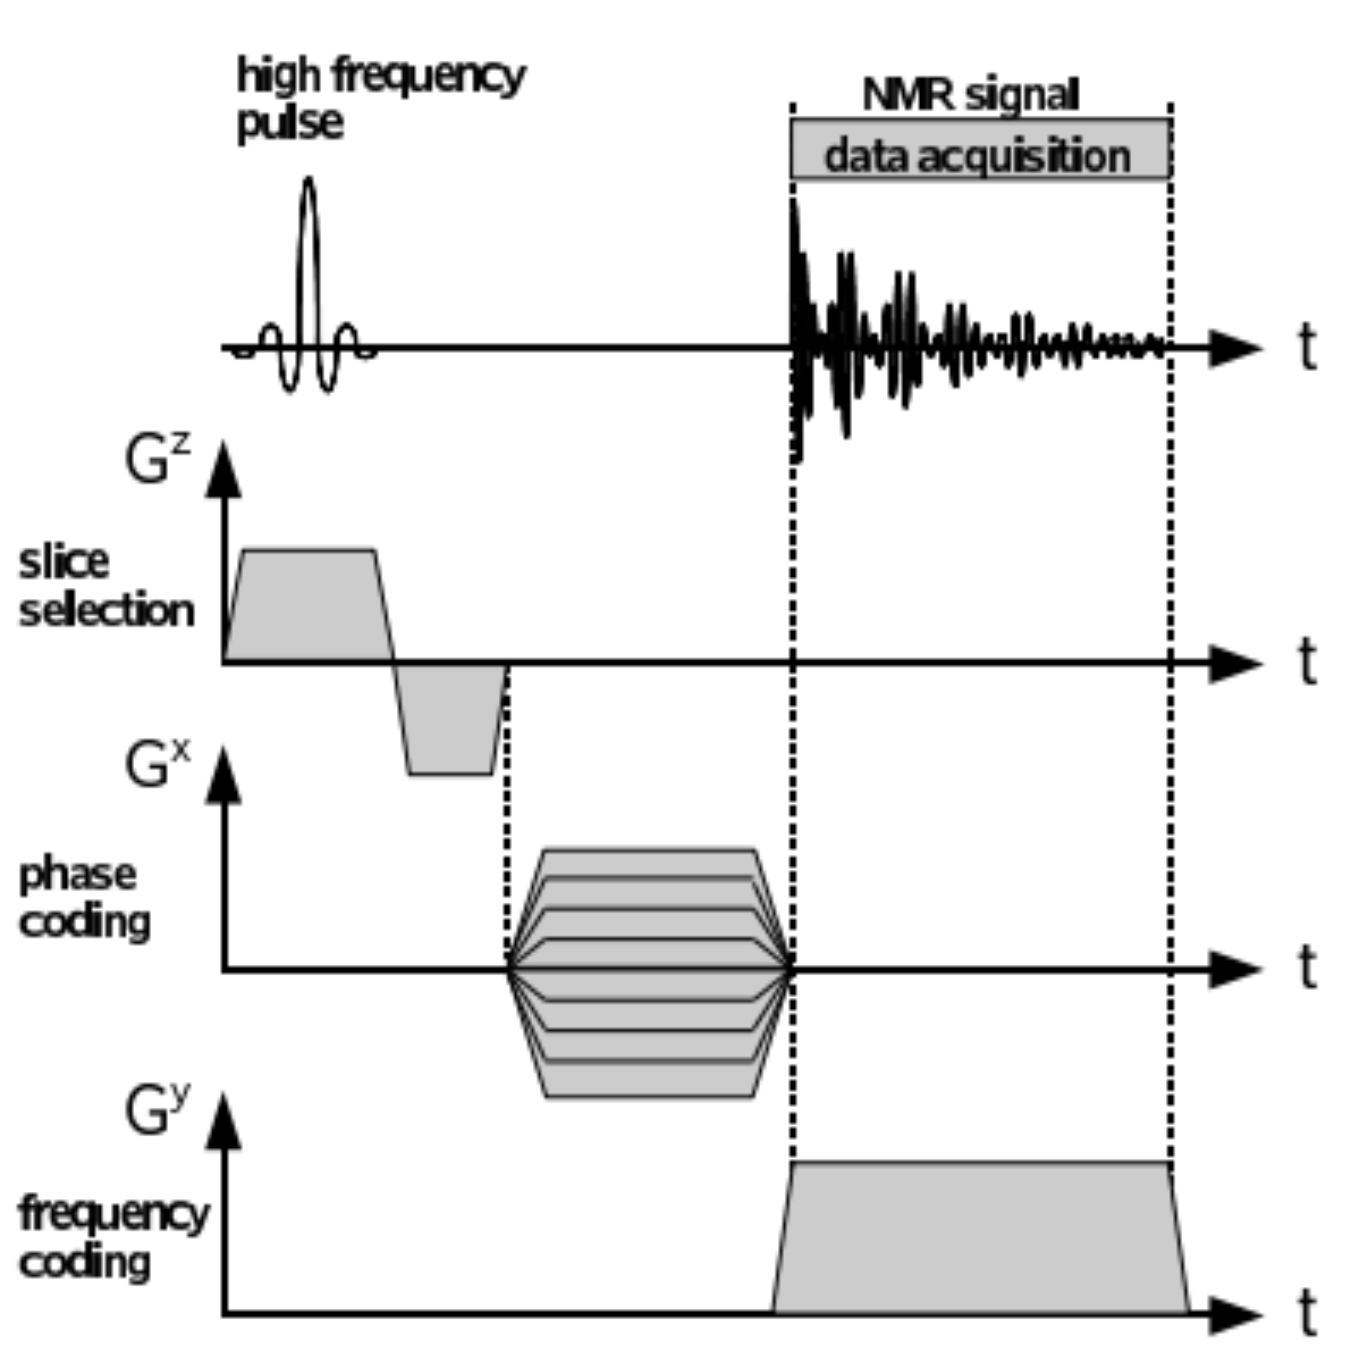
\includegraphics[scale=.25]{images//signal.png}
\caption{Datarecording for two dimensional imaging \cite{script_nmr}.}
\label{fig:signal}
\end{figure}
It is obvious that by stimulating individual layers and creating the respective images one after the other, three-dimensional objects can also be examined.